
\begin{wrapfigure}{r}{0.5\textwidth}
  \begin{center}
    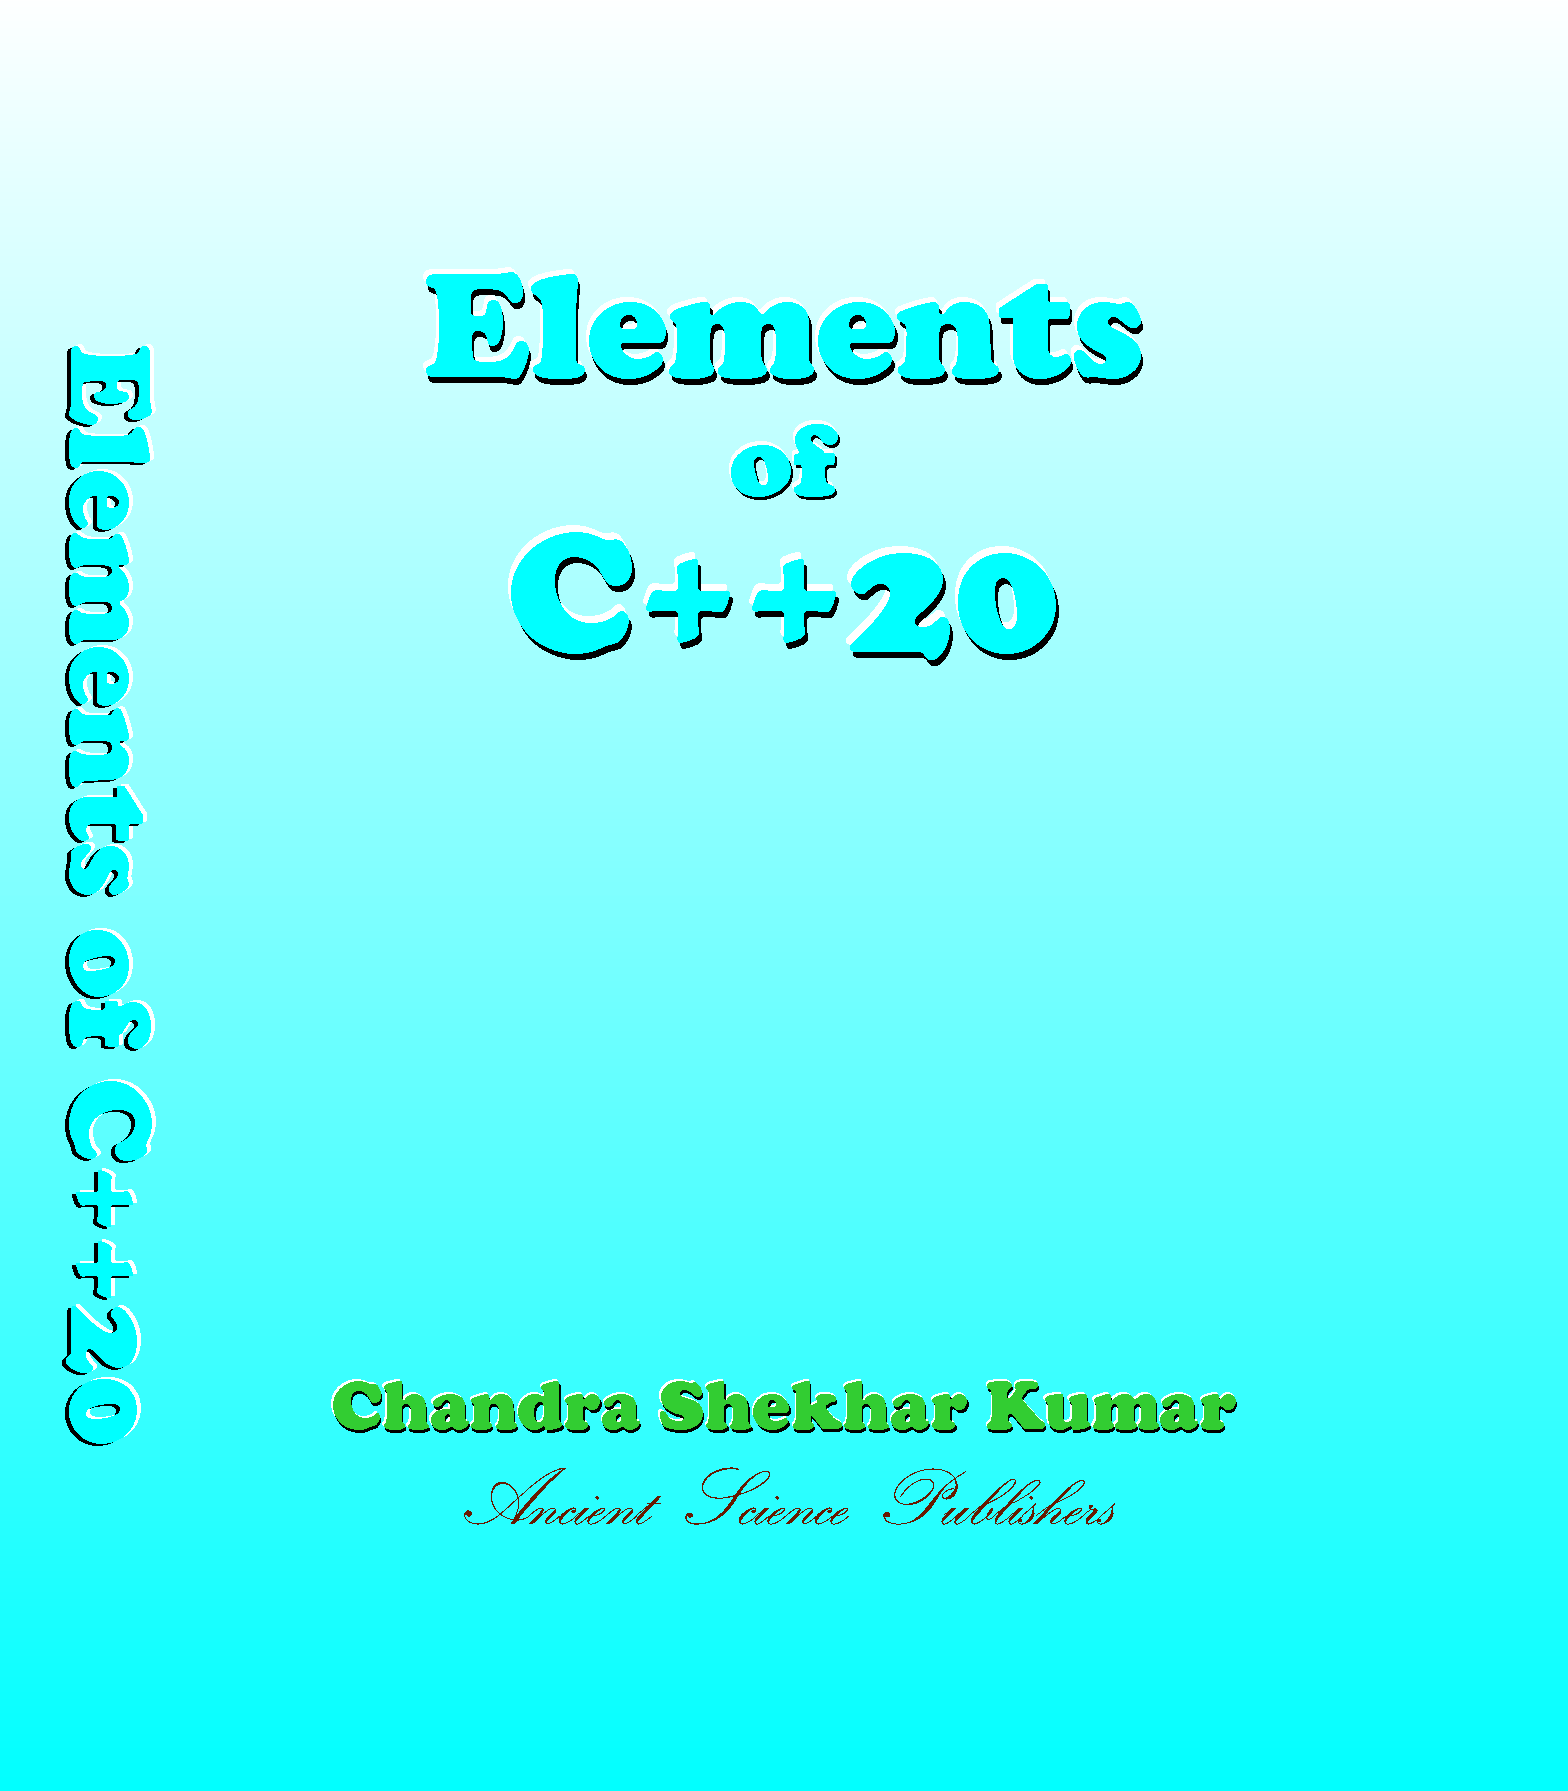
\includegraphics[width=0.5\textwidth]{cpp20/cover}
  \end{center}
  %\caption{Front Cover}
\end{wrapfigure}

\hspace{5mm}This book is a rigorous treatment of salient features of C++ 20 language and library in line with ISO/IEC standard to suit the needs of practicing professionals and experts alike. Armed with \textbf{2000+} examples and 1000+ indices with emphasis on standard library with indicative approach to implementation, it stands as a quick reference too for important concepts. 

\vspace{2mm}

I am grateful for this opportunity to put the materials into a consistent format, and to correct errors in the original ISO/IEC draft that have come to my attention. The process of compiling this book has given me an incentive to improve and extend the text, concepts, problems, solutions, layout, to double check almost all of the mathematical rendering, to correct all known errors, to improve the original illustrations by redrawing them with Till Tantau's marvellous \textup{Ti\textit{k}Z}, to include new diagrams. Thus the book now appears in a form that I hope will remain useful for at least another decade.

\section{Table of Contents}
\setlist{nosep}
\begin{enumerate}%[label*=\arabic*.]
\item Modules
    \begin{enumerate}[label=\arabic{enumi}.\arabic*., itemindent=!]
      \item Module units and purviews
      \item Export declaration 
      \item Import declaration 
      \item Global module fragment 
      \item Private module fragment 
      \item Instantiation context 
      \item Reachability
    \end{enumerate}
\item Classes
    \begin{enumerate}[label=\arabic{enumi}.\arabic*., leftmargin=*]
      \item Preamble   
      \item Properties of classes 
      \item Class names 
      \item Class members 
      \item Unions 
      \item Local class declarations
      \item Derived classes 
      \item Member access control 
      \item Initialization 
      \item Comparisons 
      \item Free store
    \end{enumerate}
\item Overloading
    \begin{enumerate}[label=\arabic{enumi}.\arabic*., leftmargin=*]
      \item Preamble 
      \item Overload resolution 
      \item Address of an overload set
      \item Overloaded operators 
      \item Built-in operators 
      \item User-defined literals
    \end{enumerate}
\item Templates
    \begin{enumerate}[label=\arabic{enumi}.\arabic*.]
      \item Preamble 
      \item Template parameters 
      \item Names of template specializations 
      \item Template arguments 
      \item Template constraints 
      \item Type equivalence 
      \item Template declarations
      \item Name resolution 
      \item Template instantiation and specialization
      \item Function template specializations
    \end{enumerate}
\item Exception handling
    \begin{enumerate}[label=\arabic{enumi}.\arabic*.]
      \item Preamble 
      \item Throwing an exception 
      \item Constructors and destructors
      \item Handling an exception 
      \item Exception specifications 
      \item Special functions
     \end{enumerate}
\item Concepts library
    \begin{enumerate}[label=\arabic{enumi}.\arabic*.]
      \item General 
      \item Equality preservation 
      \item Header <concepts> synopsis 
      \item Language-related concepts 
      \item Comparison concepts 
      \item Object concepts 
      \item Callable concepts
     \end{enumerate}
\item General utilities library
    \begin{enumerate}[label=\arabic{enumi}.\arabic*.]
      \item General 
      \item Utility components 
      \item Compile-time integer sequences 
      \item Pairs 
      \item Tuples 
      \item Optional objects  
      \item Variants 
      \item Storage for any type 
      \item Bitsets 
      \item Memory 
      \item Smart pointers 
      \item Memory resources 
      \item Class template scoped\_allocator\_adaptor
      \item Function objects
      \item Metaprogramming and type traits 
      \item Compile-time rational arithmetic 
      \item Class type\_index 
      \item Execution policies 
      \item Primitive numeric conversions 
      \item Formatting 
      \item Stacktrace
     \end{enumerate}
\item Strings library
    \begin{enumerate}[label=\arabic{enumi}.\arabic*.]
      \item General 
      \item Character traits 
      \item String classes
      \item String view classes
      \item Null-terminated sequence utilities
     \end{enumerate}
\item Containers library
    \begin{enumerate}[label=\arabic{enumi}.\arabic*.]
      \item General 
      \item Container requirements
      \item Sequence containers 
      \item Associative containers 
      \item Unordered associative containers
      \item Container adaptors 
      \item Views
     \end{enumerate}
\item Iterators library
    \begin{enumerate}[label=\arabic{enumi}.\arabic*.]
      \item General 
      \item Header <iterator> synopsis
      \item Iterator requirements 
      \item Iterator primitives 
      \item  Iterator adaptors 
      \item Stream iterators 
      \item  Range access
     \end{enumerate}
\item Ranges library
    \begin{enumerate}[label=\arabic{enumi}.\arabic*.]
      \item General       
      \item Header <ranges> synopsis
      \item Range access 
      \item Range requirements 
      \item Range utilities 
      \item Range factories 
      \item Range adaptors
     \end{enumerate}
\item Algorithms library
    \begin{enumerate}[label=\arabic{enumi}.\arabic*.]
      \item  General 
      \item  Algorithms requirements 
      \item Parallel algorithms 
      \item Header <algorithm> synopsis 
      \item Algorithm result types 
      \item Non-modifying sequence operations
      \item  Mutating sequence operations 
      \item Sorting and related operations 
      \item Header <numeric> synopsis 
      \item Generalized numeric operations 
      \item Specialized <memory> algorithms 
      \item C library algorithms
     \end{enumerate}
\end{enumerate}      
      
      
      
      
      
      
      